\documentclass[11pt,aspectratio=43]{beamer}
\usepackage[utf8]{inputenc}
\usepackage{amsmath, amsfonts, amssymb, amsthm}
\usepackage[T1]{fontenc}
\usepackage{lmodern}
\usepackage{xcolor}
\usepackage{setspace}
\usepackage{booktabs}
\usepackage{multirow}
\usepackage{graphicx}
\usepackage{tikz}
% \usetikzlibrary{decorations}
\usetikzlibrary{decorations.pathreplacing}
\usepackage{ulem}
\usepackage{hyperref}
\usepackage{booktabs}
\usepackage{babel}
\usepackage{makecell}
\usepackage[para,online,flushleft]{threeparttable}
\usepackage{pdfpages}
\usepackage{tcolorbox}
\usepackage{bm}
\usepackage{appendixnumberbeamer}
\usepackage{natbib}
\usepackage{caption}
\captionsetup[figure]{labelformat=empty}% redefines the caption setup of the figures environment in the beamer class.
\usetheme[compress]{Boadilla}
\usecolortheme{default}
\useoutertheme{miniframes}
\usefonttheme[onlymath]{serif}

\newcommand{\jump}[2]{\hyperlink{#1}{\beamerbutton{#2}}}
\newcommand{\orange}[1]{\textcolor{orange}{#1}}
\newcommand{\red}[1]{\textcolor{red}{#1}}

\setbeamertemplate{itemize item}{\raisebox{0.1em}{\scalebox{0.7}{$\blacksquare$}}}
\setbeamertemplate{itemize subitem}[circle]
\setbeamertemplate{itemize subsubitem}{--}
\setbeamercolor{itemize item}{fg=black}
\setbeamercolor{itemize subitem}{fg=black}
\setbeamercolor{itemize subsubitem}{fg=black}
\setbeamercolor{item projected}{bg=darkgray,fg=white}
\definecolor{blue}{rgb}{0.2, 0.2, 0.7}
\setbeamercolor{alerted text}{fg=blue}
\setbeamertemplate{enumerate items}[circle]


\setbeamertemplate{headline}{}

%==========================================
\let\olditemize=\itemize
\let\endolditemize=\enditemize
\renewenvironment{itemize}{\olditemize \itemsep1em}{\endolditemize}
\let\oldenumerate=\enumerate
\let\endoldenumerate=\endenumerate
\renewenvironment{enumerate}{\oldenumerate \itemsep1em}{ \endoldenumerate}

\DeclareMathOperator*{\argmax}{\arg\!\max}
\DeclareMathOperator*{\E}{\mathbb{E}}
\DeclareMathOperator*{\var}{\rm Var}
\DeclareMathOperator*{\cov}{\rm Cov}

\theoremstyle{definition}
\newtheorem{assume}{Assumption}
\newtheorem{lem}{Lemma}
\newtheorem{proposition}{Proposition}
\newtheorem{thm}{Theorem}
\newtheorem{corol}{Corollary}

\begin{document}
    \title[Lecture 17]{Lecture 17 \\ The Real Business Cycle Model \\ Part 4: Formal Examples}
    \author[Hui-Jun Chen]{Hui-Jun Chen}
    \institute[OSU]{The Ohio State University}
    % \date{\today}
    \date[\today]{\today \\ Credit: Kyle Dempsey}
    \setbeamertemplate{navigation symbols}{}
    \setstretch{1.2}

%-------------------------------------------------------
{
%	\usebackgroundtemplate{\includegraphics[width=1\paperwidth]{../EveningSky_cropped_edit43_bright.jpg}}
    \begin{frame}
% \vspace{3em}
        \centering
%		{\footnotesize 	ECON 4002 Intermediate Macroeconomic Theory}
        \maketitle
% \vspace{-1.5em}
% \centering
% \includegraphics[width=0.55\linewidth]{Pictures/houses.jpeg}


    \end{frame}
}

% -------------------------------------------
\setbeamertemplate{headline}
{
\setbeamercolor{section in head/foot}{fg=black, bg=white}
\vskip1em \tiny \insertsectionnavigationhorizontal{1\paperwidth}{\hspace{0.50\paperwidth}}{}
}
%------------------------------------------


\begin{frame}{Overview}
\label{slide:Overview}
    \begin{itemize}
        \item Recall that in Lecture 13, there is no production in dynamic model.
        \item The following $ 5 $ lectures is for \textbf{Real Business Cycle} (RBC) model:
        \begin{itemize}
            \item Lecture 14: consumer
            \item Lecture 15: firm
            \item Lecture 16: competitive equilibrium
            \item Lecture 17: formal example
            \item Lecture 18: application to bring RBC to data
        \end{itemize}
    \end{itemize}
\end{frame}

\section{Setup}
\label{sec:Setup}

\begin{frame}{Assumptions}
\label{slide:Assumptions}
    \begin{itemize}
        \item \textbf{consumer}: assume discounting factor $ \beta \in ( 0, 1 ) $ and utility function is
        \begin{center}
            $ \displaystyle \tilde{U}( C, N, C') = \ln C + \beta \ln C' + \gamma \ln ( 1-N ),$
        \end{center}
        where $ \gamma > 0 $, and consumer endowed with $ 1 $ unit of time.
        \begin{itemize}
            \item we assume no dis-utility in date 1 labor supply to simplify analysis
        \end{itemize}
        \item \textbf{firm}: assume production is Cobb-Douglas in both periods:
        \begin{center}
            $ \displaystyle Y = z K^{\alpha} N^{1-\alpha} $ and $ \displaystyle Y' = z' K'^{\alpha} N'^{1-\alpha} $,
        \end{center}
        where $ K $ is initial capital, TFP $ z = 1 $, and depreciation $ \delta \in ( 0, 1 ) $
        \item \textbf{government}: spend $ G $ and $ G' $, which is financed by lump-sum taxes $ T, T' $ and deficit $ B $
    \end{itemize}
\end{frame}

\begin{frame}{Competitive Equilibrium}
\label{slide:Competitive_Equilibrium}
    \scriptsize
    Given exogenous quantities $ \{ G, G', z, z', K \} $, a competitive equilibrium is a set of (1) consumer choices $ \{ C, C', N_{S}, N'_{S}, l, l', S \} $; (2) firm choices $ \{ Y, Y', \pi, \pi', N_{D}, N'_{D}, I, K' \} $; (3) government choices $ \{ T, T', B \} $, and (4) prices $ \{ w, w', r \} $ such that
    \begin{enumerate}
        \item Taken $ \{ w, w', r, \pi, \pi' \} $ as given, consumer chooses $ \{ C', N_{S}, N'_{S} \} $ to solve
            %
            \begin{center}
                $
                \displaystyle
                \max_{C', N_{S}, N'_{S}} \ln \left(
                    w N_{S} + \pi - T +
                    \frac{w' N'_{S} + \pi' - T' - C'}{1+r}
                \right) + \beta \ln C' + \gamma \ln ( 1-N_{S} )
                $,
            \end{center}
            where we can back out $ \{ C, S, l, l' \} $.
        \item Taken $ \{ w, w', r \} $ as given, firm chooses $ \{ N_{D}, N'_{D}, K' \} $ to solve
            %
            \begin{center}
                $
                \displaystyle
                \max_{N_{D}, N'_{D}, K'} z K^{\alpha} N_{D}^{1-\alpha} - w N_{D} - [ K' - ( 1-\delta ) K ] + \frac{z' ( K' )^{\alpha}( N'_{D} )^{1-\alpha} - w' N'_{D} + ( 1-\delta ) K'}{1+r}
                $,
            \end{center}
            where we can back out $ \{ Y, Y', \pi, \pi', I \} $.
        \item Taxes and deficit satisfy $ \displaystyle T + \frac{T'}{1+r} = G + \frac{G'}{1+r} $ and $ G - T = B $.
        \item All markets clear: (i) labor, $ N_{S} = N_{D} $ \& $ N'_{S} = N'_{D} $; (ii) goods, $ Y = C + G $ \& $Y' = C' + G' $; (iii) bonds at date 0, $ S = B $.
    \end{enumerate}
\end{frame}

\section{Labor Market}
\label{sec:Labor_Market}

\begin{frame}{Step 0: Result Implied by Assumptions}
\label{slide:Step_0__Result_Implied_by_Assumptions}
    \begin{enumerate}
        \item $ N'_{S} = 1 $, since consumer don't value leisure at date 1.
        \begin{itemize}
            \item If consumer don't value leisure, then choose the highest possible $ N'_{S} $ can expand the budget set without decreasing the utility.
        \end{itemize}
        \item $ N'_{D} = N'_{S} = 1 $, by future labor market clearing.
        \item The future wage $ w' $ is determined by $ MPN' $:
        %
        \begin{equation*}
            MPN' = z ( 1-\alpha ) \left(
                \frac{K'}{N'_{D}}
            \right)^{\alpha}
        ,\end{equation*}
        %
        where $ N'_{D} = 1 $ leads to
        %
        \begin{equation*}
            w' = z ( 1-\alpha ) ( K' )^{\alpha}
        .\end{equation*}
        %
    \end{enumerate}
\end{frame}

\begin{frame}{Step 1: Firm's Current Labor Demand}
\label{slide:Step_1__Firm_s_Current_Labor_Demand}
    \begin{columns}
        \begin{column}{0.5\textwidth}
            \begin{figure}
                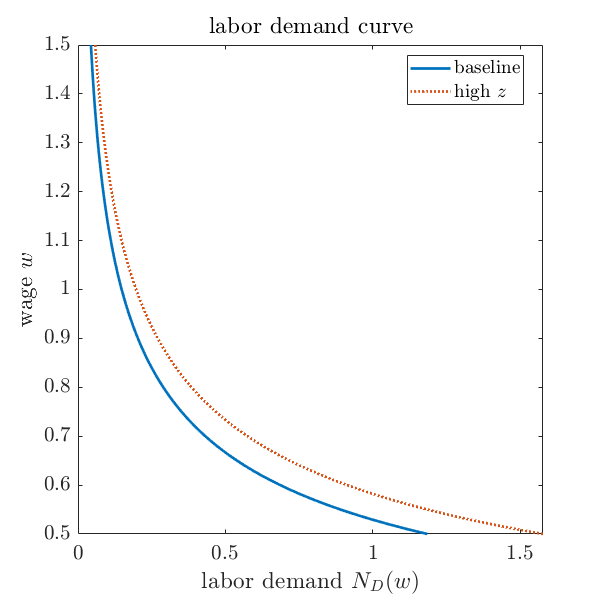
\includegraphics[width=\textwidth]{./figures/LaborDemandTFP.png}
            \end{figure}
        \end{column}
        \begin{column}{0.5\textwidth}
            For date 0 labor demand,
            %
            \begin{align*}
                MPN
                    & = z ( 1-\alpha ) \left(
                        \frac{K}{ N_{D}}
                    \right)^{\alpha} = w
                \\
                \Rightarrow N_{D}
                    & = \left(
                        \frac{z ( 1-\alpha )}{w}
                    \right)^{\frac{1}{\alpha}} K
            \end{align*}
            %
            \begin{itemize}
                \item $ N_{D} \downarrow $ in current wage $ w $
                \item $ N_{D} \uparrow  $ in current TFP $ z $ (dotted line)
                \item $ N_{D} $ invariant to interest rate
            \end{itemize}
        \end{column}
    \end{columns}
\end{frame}

\begin{frame}{Step 2: Consumer \& Current Labor Supply}
\label{slide:Step_2__Consumer_Analysis}
    \begin{itemize}
        \item \alert{labor supply} at date 0:
        %
        \begin{align*}
           MRS_{l, C}
                & = -MRS_{N, C} = -\frac{D_{N} \tilde{U}( \cdot )}{D_{C} \tilde{U}( \cdot )}
            \\
                & = -\frac{-\gamma/( 1-N_{S} )}{1/C} = \frac{\gamma C}{1-N_{S}} = w
        \end{align*}
        %
        \item \alert{Saving} at date 0:
        %
        \begin{equation*}
            MRS_{C, C'} = \frac{1/C}{\beta/C'} = \frac{C'}{\beta C} = 1+r \Rightarrow C' = \beta( 1+r ) C
        \end{equation*}
        %
        \item Recall $ N'_{S} = 1$, we can denote the $ x $ notation to be the part of the income that is NOT \alert{directly affected by consumer choice}:
        %
        \begin{equation*}
            x = \pi - T \quad \text{and} \quad x' = w' + \pi' - T'
        \end{equation*}
        %
    \end{itemize}
\end{frame}

\begin{frame}{Step 2: Consumer \& Current Labor Supply (Cont.)}
\label{slide:Step_2__Consumer_Analysis_for_Current_Labor_Supply__Cont__}
\footnotesize
Recall consumer budget constraint,
%
\begin{align*}
    C + \frac{C'}{1+r}
        & = w N_{S} + \pi - T
        + \frac{ w' N'_{S} + \pi' - T' }{1+r}
    \\
    C + \frac{\beta( 1+r )C}{1+r}
        & = wN_{S} + x + \frac{x'}{1+r}
    \\
    C
        & = \frac{1}{1+\beta}
            \left(
                w N_{S} + x + \frac{x'}{1+r}
            \right)
\end{align*}
%
plug back to labor supply condition:
%
\begin{align*}
    w( 1-N_{S} )
        & = \gamma C
    \\
    w( 1-N_{S} )
        &= \frac{\gamma}{1+\beta}
            \left(
                w N_{S} + x + \frac{x'}{1+r}
            \right)
    \\
    w N_{S} \left(
        \frac{\gamma}{1+\beta} + 1
    \right)
        & = w - \frac{\gamma}{1+\beta} \left(
            x + \frac{x'}{1+r}
        \right)
    \\
    N_{S}
        &= \frac{1+\beta}{1+\beta+\gamma} - \frac{1}{w} \frac{\gamma}{1+\beta+\gamma}\left(
            x + \frac{x'}{1+r}
        \right)
\end{align*}
%
\end{frame}

\begin{frame}{Check: Labor Supply Assumptions}
\label{slide:Check__Labor_Supply_Assumptions}
    \begin{columns}
        \begin{column}{0.5\textwidth}
            \begin{figure}
                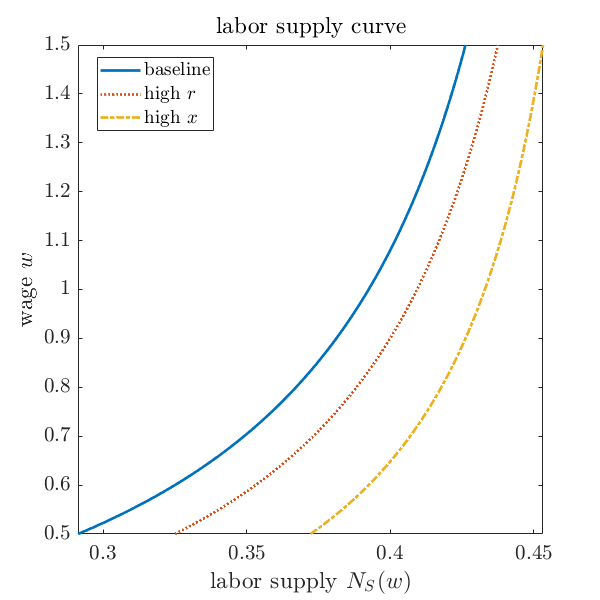
\includegraphics[width=\textwidth]{./figures/LaborSupplyInterestRateWealth.png}
            \end{figure}


        \end{column}
        \begin{column}{0.5\textwidth}
            Recall \textbf{N1}-\textbf{N3} assumptions,
            \begin{itemize}
                \item \textbf{N1}: labor supply $ \uparrow  $ in wage, $ d N_{S} / dw > 0 $ (all lines)
                \item \textbf{N2}: labor supply $ \uparrow  $ in real interest rate, $ d N_{S} / dr > 0 $ (red v.s. blue)
                \item \textbf{N3}: labor supply $ \downarrow  $ in lifetime wealth, $ d N_{S} / d( x + x' ) < 0 $ (yellow v.s. blue)
            \end{itemize}
        \end{column}
    \end{columns}
\end{frame}

\begin{frame}{Check: Labor Market Clearing}
\label{slide:Check__Labor_Market_Clearing}
    \begin{columns}
        \begin{column}{0.5\textwidth}
            \begin{figure}
                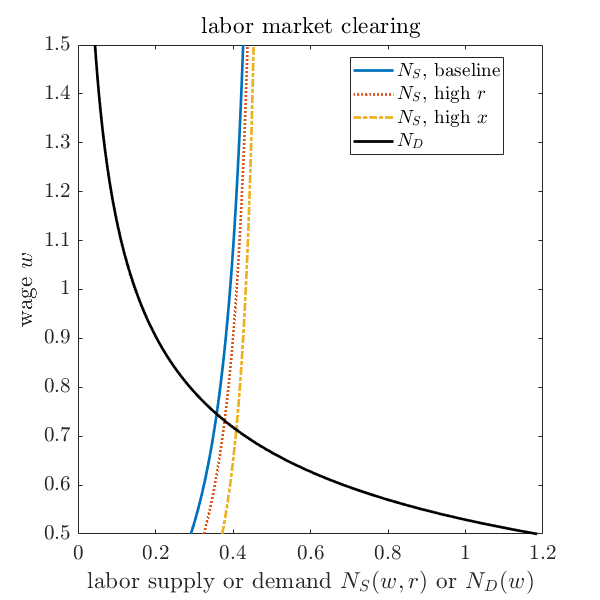
\includegraphics[width=\textwidth]{./figures/LaborMarketClear.png}
            \end{figure}
        \end{column}
        \begin{column}{0.5\textwidth}
            higher interest rate (\textbf{N2}), lower lifetime wealth (\textbf{N3}) both shifts out labor supply curve:
            \begin{itemize}
                \item wage $ w^{*}( r ) $ increases
                \item equilibrium quantity of labor $ N^{*}( r ) $ decreases
            \end{itemize}
            Next: construct output supply curve
        \end{column}
    \end{columns}
\end{frame}

\section{Output Market}
\label{sec:Output_Market}

\begin{frame}{Step 3: Output Supply Curve}
\label{slide:Step_3__Output_Supply_Curve}
    Labor market clearing requires:
    %
    \begin{equation*}
        N_{S} = \frac{1+\beta}{1+\beta+\gamma} - \frac{1}{w} \frac{\gamma}{1+\beta+\gamma}
                \left(
                    x + \frac{x'}{1+r}
                \right)
                =
                \left(
                    \frac{z ( 1-\alpha )}{w}
                \right)^{\frac{1}{\alpha}}
                = N_{D}
    .\end{equation*}
    %
    ...Yeah, it is very difficult to solve it by hand (actually cannot), but notice
    \begin{itemize}
        \item most of the terms are parameters: $ \alpha, \beta, \gamma, z, K $,
        \item or lifetime wealth that needs gov: $ x $ and $ x' $.
        \item Out main goal is to \alert{solve for $ w^{*}( r ) $!}
        \begin{itemize}
            \item solve real wage $ w $ as a function of real interest rate $ r $
            \item then, back out $ N^{*}( r ) $ and $ Y_{S}( r ) $
            \begin{itemize}
                \item get $ N^{*}( r ) $ by plug $ w^{*}( r ) $ into either $ N_{D} $ or $ N_{S} $
                \item get $ Y_{S}( r ) $ by plug $ N^{*}( r ) $ into $ z K^{\alpha} ( N^{*} )^{1-\alpha} $
            \end{itemize}
        \end{itemize}
    \end{itemize}
\end{frame}

\begin{frame}{Check: Output Supply Curve}
\label{slide:Check__Output_Supply_Curve}
    \begin{figure}
        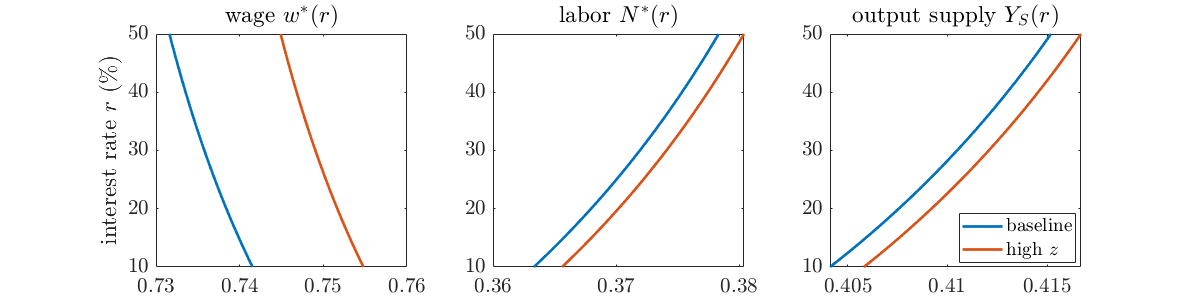
\includegraphics[width=\textwidth]{./figures/OutputSupply.png}
    \end{figure}
    Confirm our intuition:
    \begin{itemize}
        \item $ r \uparrow  $ leads to $ w \downarrow  $ and $ N^{*}( r ) \uparrow  $
        \item given positive $ MPN $ and fixed $ K $, more labor means more production, so output supply shifts up.
    \end{itemize}
\end{frame}

\begin{frame}{Step 4: Output Demand Curve}
\label{slide:Step_4__Output_Demand_Curve}
    Recall that the date 0 output demand curve are composite of
    \begin{itemize}
        \item government spending $ G $ and $ G' $: exogenous (easy!)
        \item firm's investment demand $ I_{D}( r ) $ (next slide)
        \item consumer's consumption demand $ C_{D}( r, Y ) $:
        \begin{itemize}
            \item recall \textbf{income-expenditure identity}, total income $ = $ total demand,
            %
            \begin{align*}
                C + \frac{C'}{1+r}
                    &  = wN + \pi - T + \frac{w' N' + \pi' - T'}{1+r}
                \\
                    & \because \pi = Y - wN - I; \pi' = Y' - w'N' + ( 1-\delta )K'
                \\
                ( 1+\beta ) C
                    & = Y + \frac{Y'}{1+r} - I + \frac{( 1-\delta )K'}{1+r} - \left( T + \frac{T'}{1+r} \right)
            \end{align*}
            %
            \item given $ r $, we can solve consumption-saving problem.
        \end{itemize}
    \end{itemize}
\end{frame}

\begin{frame}{Firm's Optimal Investment}
\label{slide:Firm_s_Optimal_Investment}
    Recall
    \begin{itemize}
        \item labor market clearing at date 1: $ N'_{D} = N'_{S} = N' = 1 $, and
        \item $ MPK $ at date 1: $ MPK' = z' \alpha ( K' )^{\alpha-1}$.
    \end{itemize}
    Thus, according to optimal investment schedule,
    %
    \begin{align*}
        MPK' - d
            &= r
        \\
        z' \alpha ( K' )^{\alpha-1}
            &=  r + d
        \\
        K'
            &= \left(
                \frac{z' \alpha}{r+d}
            \right)^{\frac{1}{1-\alpha}}
    \end{align*}
    %
    and we can also determine investment by capital accumulation process:
    %
    \begin{equation*}
        I_{D} = K' - ( 1-\delta)K
          = \left(
                \frac{z' \alpha}{r+d}
            \right)^{\frac{1}{1-\alpha}}
            - ( 1-\delta )K
    \end{equation*}
    %
\end{frame}

\begin{frame}{Check: Investment Demand Assumption}
\label{slide:Check__Investment_Demand_Assumption}
    \begin{columns}
        \begin{column}{0.5\textwidth}
            \begin{figure}
                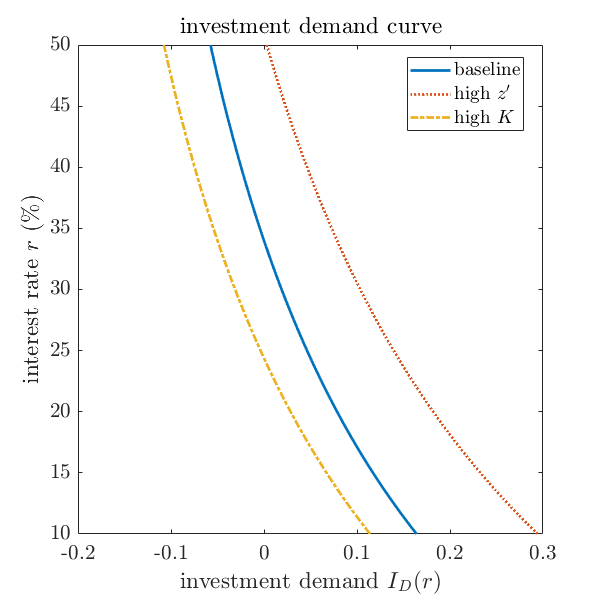
\includegraphics[width=\textwidth]{./figures/InvestmentDemand.png}
            \end{figure}
        \end{column}
        \begin{column}{0.5\textwidth}
            \begin{center}
                $ \displaystyle
                I_{D} = \left(
                        \frac{z' \alpha}{r+d}
                    \right)^{\frac{1}{1-\alpha}}
                    - ( 1-\delta )K
                $
            \end{center}
            Recall assumptions from Lecture 15:
            \begin{itemize}
                \item $ I_{D}( r ) \downarrow $ in $ r $ ($\checkmark$)
                \item $ I_{D}( r ) $ shifts in when $ K \uparrow $: yellow v.s. blue
                \item $ I_{D}( r ) $ shifts out when $ z' \uparrow  $: red v.s. blue
            \end{itemize}
        \end{column}
    \end{columns}
\end{frame}

\begin{frame}{Constructing the Output Demand Curve}
\label{slide:Constructing_the_Output_Demand_Curve}
    \begin{columns}
        \begin{column}{0.5\textwidth}
            \begin{figure}
                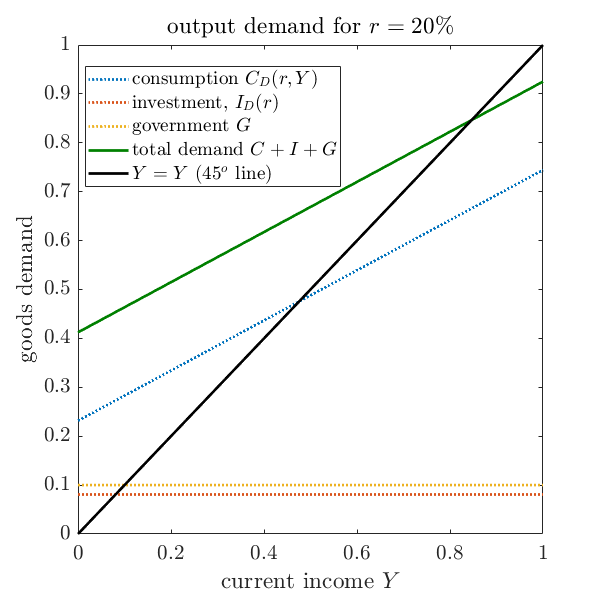
\includegraphics[width=\textwidth]{./figures/OutputDemand.png}
            \end{figure}


        \end{column}
        \begin{column}{0.5\textwidth}
            Aggregate all three components:
            \begin{itemize}
                \item investment (red) and government (yellow) are horizontal
                \item consumption (blue) increase in income with slope $ \approx \frac{1}{1+\beta} $
                \item total output demand (green) gain the slope from consumption, and is the sum of all three
            \end{itemize}
        \end{column}
    \end{columns}
\end{frame}

\begin{frame}{Constructing the Output Demand Curve (Cont.)}
\label{slide:Constructing_the_Output_Demand_Curve__Cont__}
    \begin{center}
        $ r \uparrow  $ $ \Rightarrow  $ $ I_{D}( r ) \downarrow  $ $ \Rightarrow  $ total demand $ \downarrow  $
    \end{center}

    \begin{columns}
        \begin{column}{0.55\textwidth}
            \begin{figure}
                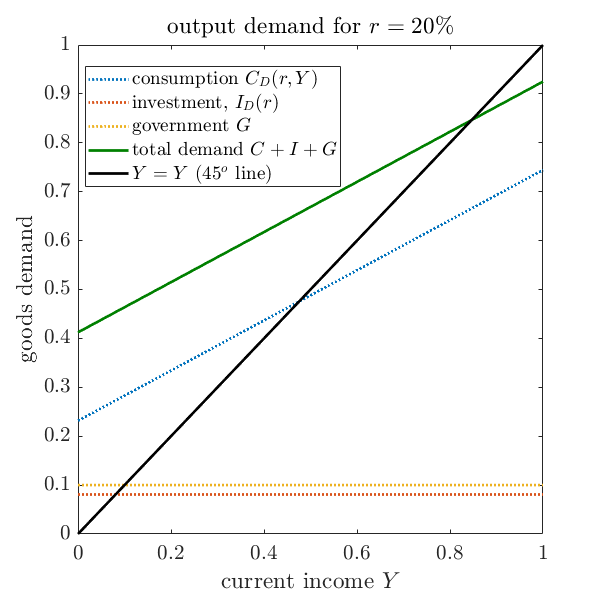
\includegraphics[width=\textwidth]{./figures/OutputDemand.png}
            \end{figure}
        \end{column}
        \begin{column}{0.55\textwidth}
            \begin{figure}
                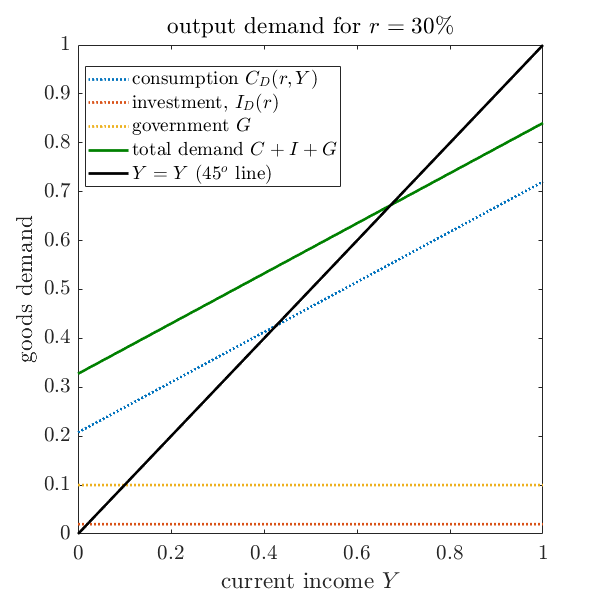
\includegraphics[width=\textwidth]{./figures/OutputDemand_2.png}
            \end{figure}
        \end{column}
    \end{columns}
\end{frame}

\end{document}


